\documentclass[10pt,compsoc]{IEEEtran}
\usepackage[spanish]{babel}
\usepackage{amsmath, amsfonts}
\usepackage{algorithmic}
\usepackage{array}
\usepackage[caption=false,font=normalsize,labelfont=sf,textfont=sf]{subfig}
\usepackage{textcomp}
\usepackage{stfloats}
\usepackage{float}
\usepackage{url}
\usepackage{verbatim}
\usepackage{graphicx}
\usepackage{balance}
\usepackage{xcolor}
\usepackage[colorlinks, urlcolor=blue]{hyperref}   

\hyphenation{op-tical net-works semi-conduc-tor IEEE-Xplore}
\def\BibTeX{{\rm B\kern-.05em{\sc i\kern-.025em b}\kern-.08em
		T\kern-.1667em\lower.7ex\hbox{E}\kern-.125emX}}

\begin{document}
	\title{El procesador CELL, desde un enfoque
		histórico}
	\author{Ramiro Barcala Roca, Valentin Angrigiani, Gabriel Hackl}
		
	\markboth{Organizacion del Computador, Catedra Marchi, 2024}%
	{How to Use the IEEEtran \LaTeX \ Templates}
	\maketitle
	
	\begin{abstract}
		Este trabajo trata sobre el procesador CELL de Sony. Se toma un enfoque investigativo y contrastante entre arquitecturas del CELL, y otras de la época (y la actualidad). Las aplicaciones principales para las que fue diseñado, y las que se descubrieron luego, junto con su importancia histórica. También veremos conceptos básicos sobre la computación heterogénea (distintos nucleos) y un análisis a futuro relacionándolo con lo anterior.
	\end{abstract}
	
	\begin{IEEEkeywords}
		SPE, PPE, SIMD, Pipeline/ing, Paralelismo, Calculos vectoriales, Computacion heterogenea, Celdas.
	\end{IEEEkeywords}
	
	\section{Introducción}
	\IEEEPARstart{A} mediados de los 2000, mientras los CPU's multinucleo recien se estaban introduciendo al mercado, la empresa Sony empieza a investigar y desarrollar su sistema de entretenimiento \textit{PlayStation 3}. Todo esto en un mercado competitivo frente a otras marcas como Microsoft y Nintendo. Terminan diseñando un procesador multi-core, el cual tiene como particularidades los sub-núcleos. Sony tambien quería estandarizar su procesador en dispositivos de todas las gamas y usos multimedias.
	
	Sin embargo, tanto el producto como su procesador fueron un fracaso comercial, pero se descubrieron usos investigativos/científicos/economicos, entre otros.
	
	
	\section{Época Pre-CELL}
	\noindent Para ponernos en contexto, vamos a explicar la situación de las arquitecturas del momento, como de las empresas que lanzaban nuevos productos (del mismo rubro o parecido) en aquella época.
	
	\subsection{Empresas del rubro de las consolas}
	\noindent 
	En el año 2005, las siguientes empresas de consolas/videojuegos, competían en el mercado: 
	\begin{itemize}
		\item{{\bf{Sony}}: Venía de un éxito rotundo con su anterior producto: la \textit{PlayStation 2}. Tenía grandes expectativas con su nueva consola, apostando a lo grande, con nuevas funcionalidades no esenciales (Ejemplo: puertos HDMI, Blue-Ray, etc).}
		
		\item{{\bf{Microsoft}}: Venía de un éxito moderado con su primer producto: la \textit{Xbox}. En su nuevo producto, la Xbox 360, se centra en abaratar los costos y proveer servicios en línea de gran calidad. Esto les pasa factura con los problemas de hardware que tendria la consola mas adelante.}
		
		\item{{\bf{Nintendo}}: No tuvo mucho éxito en su consola anterior: la \textit{Gamecube}. En la \textit{Wii}, se decide no hacer costos de fabricación muy caros. Pero además, se centra en facilitar experiencias novedosas para el usuario final, mediante el uso de movimientos corporales para controlar los juegos, como extensiones al mismo control (volantes, soportes, etc).}
	\end{itemize}
	
	Es necesario comprender que la industria de los juegos estaba en su apogeo. No solo se estaban demandando consolas cada vez más rápidas y potentes, sino también mucha mas gente se introducía a este tipo de consumo.
	

	
	\begin{figure}[H]
	\centering
	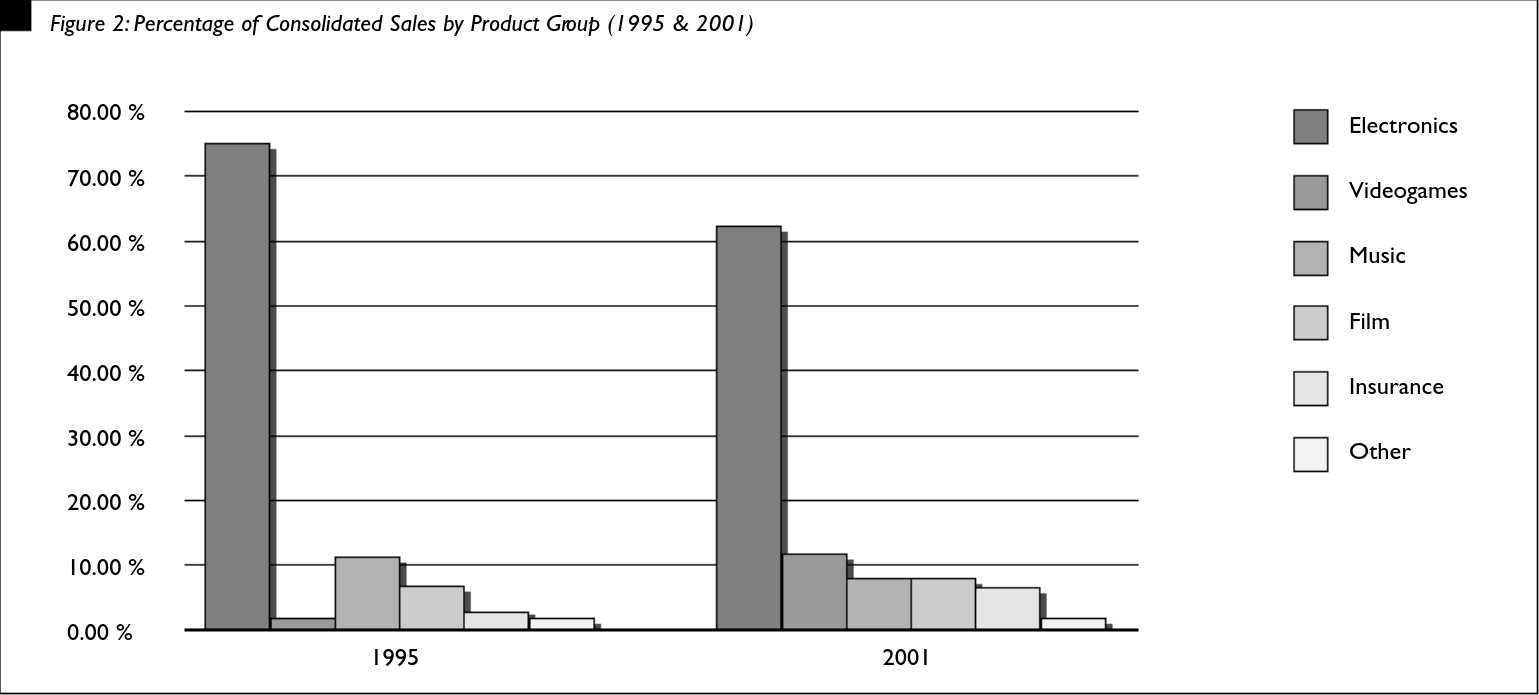
\includegraphics[width=3.5in]{imgs/gamingshare.png}
	\caption{Análisis del mercado del entretenimiento, entrando al nuevo milenio.}
	\label{fig2}
	\end{figure}
	
	

	\begin{figure}[H]
	\centering
	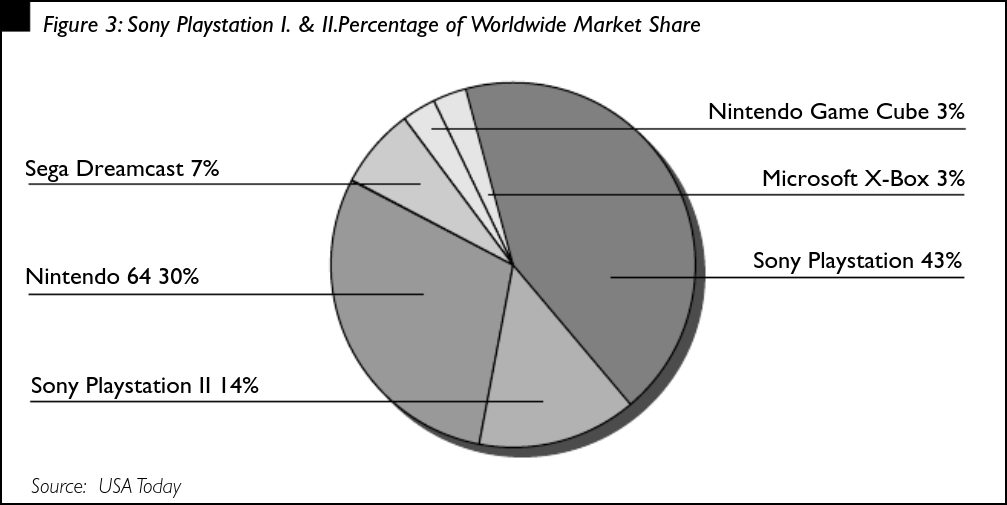
\includegraphics[width=3.5in]{imgs/marketshare.png}
	\caption{Porción del mercado de las consolas, de cada empresa.}
	\label{fig1}
	\end{figure}	
	
	
	\section{Arquitectura CELL}	% MODULOS,ARQUITECTURAS INTERNAS, CONVENCIONES, INSTRUCCIONES, etc
	\noindent Diseñada por Sony, en conjunto con Toshiba e IBM, esta arquitectura trae al mercado un procesador que maneja fuertemente la computación heterogénea, mediante el uso de sus 9 núcleos. 
	
	Si bien originalmente se pensaba incluirlo en dispositivos multimedia y del entretenimiento varios, se terminó destinando casi unicamente en la PlayStation 3. De todas formas, Sony realmente quería traer una nueva revolución al rubro del diseño de arquitecturas.
	
	\subsection{Distintos módulos del Cell} 
	\noindent Para empezar, hablaremos del PPE (\textit{Power Processing Element}). Este nucleo, es el principal de la arquitectura. Es de proposito general, y a su vez se encarga de controlar el resto de los sub-núcleos (cargar memoria y ejecutar instrucciones). Estaba conformado por una memoria caché L1 (de 64 KB), una memoria caché L2 (de 512 KB), y por el PPU (\textit{Power Processing Unit}).\newline
	
	Luego, los SPE (\textit{Synergistic Processing Element}), son los distintos sub-núcleos de la arquitectura. No son de proposito general; más bien se encargan de realizar operaciones vectoriales dirigidas desde el PPE. Cada uno tiene su memoria interna (\textit{Local Store}), un módulo \textit{Memory Flow Controller} para poder recibir/transmitir datos desde el Bús, y el SPU (\textit{Synergistic Processing Unit}).
	Cada uno de estos SPE trabajan con instrucciones SIMD con punto flotante, pudiendo llegar a realizar 25,6 Gigaflops por segundo (25,6 mil millones de operaciones de punto flotante por segundo). Vale la pena mencionar que las instrucciones SIMD se encargan de aplicar la misma operación a un conjunto de datos, para así poder obtener un mayor rendimiento en tiempo.\newline
	
	Adicionalmente cuenta con el \textit{Memory Interface Controller} (MIC, un controlador de memoria externa), y con el \textit{Bus Interface Controller} (BIC, con 2 vías de entrada y salida). En la siguiente figura podemos observar cómo están organizados los distintos módulos:
	
	\begin{figure}[H]
		\centering
		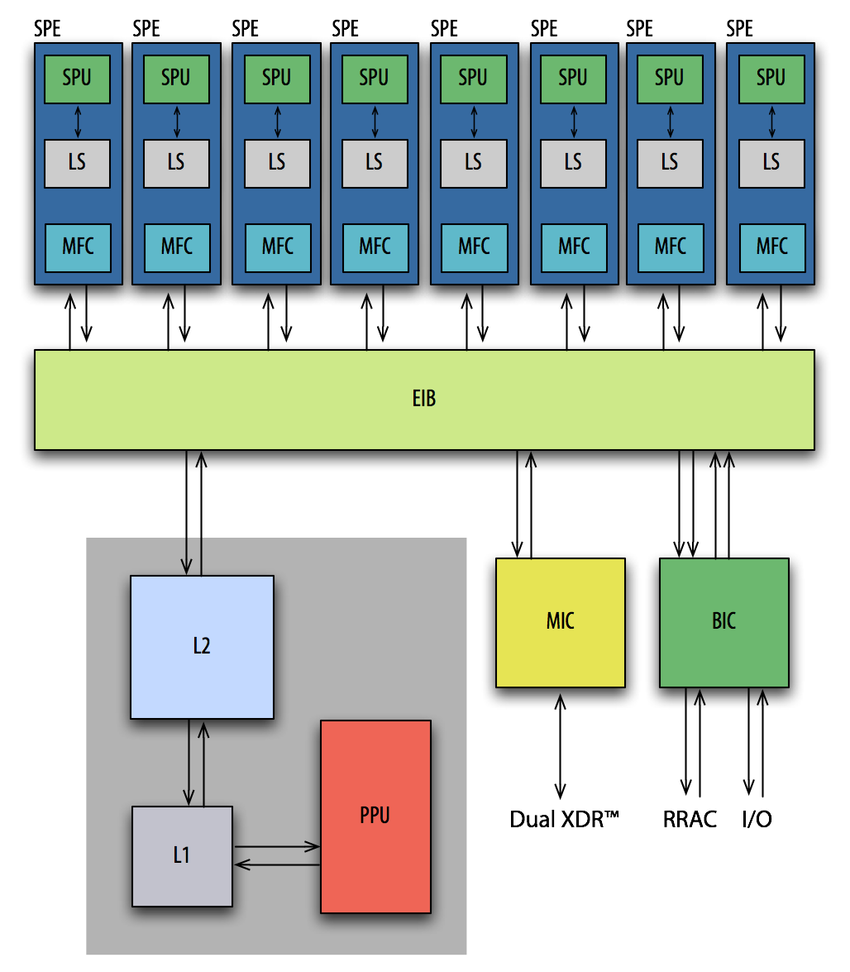
\includegraphics[width=3.2in]{imgs/arquitecturacell.png}
		\caption{Arquitectura del CELL Broadband Engine.}
		\label{fig3}
	\end{figure}
	
	\subsection{Interconexión} 
	\noindent La interconexion de los distintos módulos y núcleos (además de la memoria externa, y la interfaz I/O) se realizaba mediante el \textit{Element Interconnection Bus} (EIB), que estaba conformado por 4 anillos unidireccionales tokenizados, 2 en cada dirección. Por ende, la información no se retransmitía más de lo que debía mediante un identificador del modulo al que debía llegar la informacion. 
	Por cómo estaba armado, nunca sería posible saturar dicho bus (ancho de banda interno máximo de 204,8 GB/s).
	

	
	\subsection{Computacion heterogenea en el Cell}% SIMD
	\noindent La computacion heterogénea puede ser entendida como aquella computación que requiere el manejo y codificado de instrucciones para una arquitectura que usa distintos tipos de núcleos.\newline
	
	A gran escala, podríamos decir que la gran mayoría de consolas o computadoras orientadas al \textit{Gaming}, hoy en dia, requieren de la misma. Se debe instruccionar al CPU, GPU, etcétera. Sucede lo mismo con modelados de financiación o de computación científica, los cuales se benefician de ambos aspectos. Sin embargo, se puede dar a una escala muchísimo más chica.\newline
	
	 Resulta que la computación heterogénea, dentro del Cell, se aplica a los distintos SPE's que residen en el mismo. De forma, que no solo programamos el PPE, sino los SPE, los cuales reciben sus instrucciones (y memoria cargada) del primero mencionado. Además, el propio desarrollador puede realizar cierto tipo de \textit{pipelining}: Paralelizar los programas de los SPE, vectorizándolos y computarizando las salidas de los mismos.\newline
	 
	 El código destinado a los SPE's debe ser escrito aparte del programa del PPE, y traducido al lenguaje de máquina por compiladores específicos de SPE's.
	
	\subsection{Contraste con arquitecturas actuales}
	\noindent La idea del Cell era aplicar el tipo de arquitectura de \textit{celdas}, donde cada módulo se encarga de una tarea lo más específica posible. Así, aplicamos el lema "\textit{Divide y vencerás}", pudiendo manejar operaciones más voluminosas y complejas. También, como cada módulo funcionaba por separado, se lo podía escalar tanto como se quisiese. Esto facilitó el creado de sistemas que aplicaban este paradigma (como las supercomputadoras).\newline
	
	 Mientras que en el Cell se requería de una computación heterogénea como la mencionada anteriormente, en las arquitecturas actuales esto no es tan así (no así en los sistemas que los abarcan. Ejemplo: Computadoras dedicadas al \textit{Gaming}, ya que manejamos núcleos de distintos tipos). No están diseñadas con núcleos diferentes, a diferencia del Cell. Entonces, el enfoque al paralelizar tareas variaba; el Cell requeria de un manejo especial por parte del desarrollador (con los SPE's), mientras que hoy en día hay muchas herramientas que facilitan la división de tareas entre los núcleos.
	
	\subsection{Arquitecturas de la competencia}%ARQUITECTURAS DEL MOMENTO
	\noindent Ya habiendo explicado la arquitectura del Cell, veremos algunas de las diferencias con las de la competencia:
	
	\begin{itemize}
				
		\item{{\bf{Microsoft}}: En la Xbox 360, se diseña una arquitectura gracias a IBM que tiene ciertas similaridades con el Cell. Por empezar, el procesador de la consola era el \textit{Xenon}, de 3 núcleos, que eran PPE's como los del Cell. Sin embargo, no se encontraba en la arquitectura ningún SPE. Los PPE's, tanto como el resto de modulos, se interconectaban mediante un bús \textit{XBAR}. A grandes rasgos, es la otra companía del momento la cual también busca un acercamiento al paralelismo.}\newline
		
		\item{{\bf{Nintendo}}: En la Wii, también se recurre a IBM. Resulta que el procesador que termina ocupando esta consola (Broadway), es un \textit{rebranding} de la arquitectura ya usada por el producto anterior (la Gamecube). Esto es así ya que IBM modifica la arquitectura que le pide Nintendo, haciéndola correr a un clock mayor.\newline
		
		Por otro lado, la Wii tambien poseía un coprocesador llamado Starlet, el cual se encargaba de tareas menores como el manejo de periféricos o retrocompatibilidad con juegos de consolas anteriores, o hasta del firmware de la consola. Sin embargo, el manejo de estos dos CPU's se alejaba bastante de la computación heterogénea que requería el Cell.}
	\end{itemize}
	
	\section{Inconveniencias}
	\noindent Debido a que programar los distintos SPE's requerían mucho tiempo, una gran cantidad  de desarrolladores pasaron por alto los programas apartes que requerian los mismos, y se centraban únicamente en el PPE, que terminaba realizando todas las tareas. Esto provocaba bajos rendimientos en los programas que corría el CELL, ya que sus SPE's quedaban inutilizados.\newline
	
	Muchas tareas que se podían paralelizar, no se estaban ejecutando como debían, ni por los sub-núcleos especializados para eso. Además, los SPE's tampoco tenían \textit{branch prediction}, por lo que sentencias como if/else eran supervisadas por el PPE, asignándole más tareas.\newline
		
	Esto provocaba una performance mediocre en la mayoría de programas realizados por desarrolladores con poco conocimiento y experiencia en este paradigma. El Cell tenía potencial, pero requería un código extremadamente conciso, con pocos condicionales y que mantuviese ocupado a los 9 núcleos en todo momento.\newline
	
	Por si no era suficiente, el costo de fabricación de la consola, durante parte de los primeros 3 años del lanzamiento, rondaba alrededor de los US\$900, mientras que el precio para el consumidor final era de US\$500; sumado a que Microsoft ya había lanzado su consola hace un año atrás, ganando gran parte del mercado. Finalmente, los consumidores a los que se destinó el producto, lo rechazaban en gran medida.
	
	
	\section{Aplicaciones del CELL}
	\noindent Sin importar el resultado de la aplicación de la arquitectura, al Cell se lo utilizó para, por ejemplo:
	
	\begin{itemize}
		
		\item{{\bf{Clima}}: Ya que para replicar efectos meteorológicos como las nubes, y para procesar el inmenso volumen de información que llega desde los instrumentos usados para las distintas mediciones, requería de un sistema que pudiese realizar estas tareas intensivas. Se decidió experimentar con esta arquitectura para diseñar más adelante una solución apropiada (que solucionase también los problemas que había con el ancho de banda limitado de memoria).}\newline
		
		\item{{\bf{Modelos de simulación}}: Un gran ejemplo de esto es el \textit{RoadRunner}, una supercomputadora que llegó a operar a 1 petaflop (mil billones de operaciones de punto flotante por segundo), capaz de simular explosiones nucleares y demás cuestiones armamentísticas del gobierno de los Estados Unidos.}\newline
		
		\item{{\bf{Medicina}}: Aquí también fue útil el Cell, ya que facilita procesar la salida de las tomografías computarizadas de un uso intensivo de recursos, para reconstruir imágenes médicas en 3D.}

	\end{itemize}
	Otras aplicaciones de la arquitectura fueron en la computarización masiva de datos, en servidores, y hasta incluso en la industria petrolera y gasífera.
	
	
	\section{Remanentes del CELL en la Actualidad}%Importancia historica
	\noindent Viendo en retrospectiva, hoy se sigue aplicando hasta cierto punto parte de lo que se promovía en la arquitectura, pero a gran escala.\newline
	
	Con el diseño de celdas, ejemplos serían las telecomunicaciones, los datos móviles; siendo las distintas células las porciones de terreno con cobertura móvil, mediante las torres. O también como las plataformas funcionando en la nube, o en los sistemas como computadoras personales, consolas, etcétera. Tanto en la memoria diviéndose en celdas, o las tareas que realiza un microprocesador, encargando a los distintos núcleos distintas tareas. Por lo visto, no solo se expandió a arquitecturas, sino a sistemas que abarcan muchas más cosas.\newline
	
	Este tipo de diseño arquitectural nos permite escalar el sistema con facilidad, pudiendo aumentar la carga de trabajo sin tener que reestructurarlo por completo. También, al suceder fallas, estas se aíslan sobre el módulo erróneo y encapsula el error, para poder modularizar, y reemplazarlo con sencillez. Además facilita el paralelismo, enfocando las celdas a propósitos simples/únicos y eficientando la utilización de recursos.\newline
	
	
	Por otro lado, la computación heterogénea no se vio tan masificada en el diseño de arquitecturas, pero sí en el uso de sistemas que los abarquen. Hoy en día, interesa más el hecho de poder realizar tareas eficientemente, con arquitecturas especializadas, para después poder complementarlas en un mismo equipo, no así como se hacía en el Cell, donde se encontraban núcleos con propósitos distintos. 
		
	\section{Análisis a futuro}
	\noindent Habiendo visto las distintas aplicaciones que hay hoy en día con las arquitecturas basadas en celdas, creemos que seguirá al alza. No solo se seguirá aplicando a los diseños de microprocesadores y sistemas, sino que se expandirá a muchos de los rubros en los que hoy no se lo toma en cuenta.\newline
	
	Un ejemplo sería en la agricultura, dividiendo en parcelas los cultivos o ganados, y controlando las cosechas o animales, para revisar en cuál se debe focalizar una atención especial. O tambien en los hospitales, buscando aquellos pacientes que requieran un cuidado particular.\newline
	
	Ahora, creemos que la computación heterogénea sí tiene lugar en el futuro, pero algo similar a como pasa en la actualidad. No que se centre en el interior de los distintos diseños minimales, sino de la manera más abstracta posible.
	
	
	\section{Conclusión}
	\noindent Creemos que, si bien el enfoque que tomó Sony con su arquitectura (originalmente compartida por dispositivos varios del mundo del entretenimiento) no tuvo un éxito considerable. Fue útil para aproximarse al mundo de la computación heterogónea, y para darle otro foco a la capacidad de conseguir un mayor rendimiento en los procesadores venideros, no solo aumentando la frecuencia del \textit{clock} de los mismos.\newline
	
	Además, tuvo bastante importancia su experimento con las arquitecturas basadas en celdas, ya que le permitió a las distintas industrias que hoy en día lo aplican, ver sus beneficios.\newline
	
	
	
	\begin{thebibliography}{1}
	
			\bibitem{ams}
			{\it{Laboratorio de Arquitecturas Avanzadas con Cell y PlayStation 3}}, Universitat de València, por Fernando Pardo y Jose A. Boluda.\newline
			
			\bibitem{ams}
			{\it{The PlayStation 3 for High Performance Scientific Computing}}, University of Tennessee: Jakub Kurzak, Alfredo Buttari, Piotr Luszczek, Jack Dongarra\newline
			
			\bibitem{ams}
			{\it{The impact of IBM Cell technology on the programming paradigm in the context of computer systems	for climate and weather	models}}, Shujia Zhou, Daniel Duffy, Thomas Clune, Max Suarez, 	Samuel Williams, Milton Halem.\newline
			
			\bibitem{ams}
			{\it{Architecture of Consoles: A practical analysis by Rodrigo Copetti}}
			
			\url{https://www.copetti.org/writings/consoles/}\newline
			
			\bibitem{ams}
			{\it{Cell Technology Tackles 3D Medical Imaging Reconstruction Challenges}}
			
			\url{https://www.techbriefs.com/component/content/article/6088-
				10976-400}\newline
			
			\bibitem{ams}
			{\it{Breaking the petaflop barrier}}
			
			\url{https://www.ibm.com/history/petaflop-barrier}\newline
			
			\bibitem{ams}
			{\it{Introducing the IBM/Sony/Toshiba Cell Processor ? Part I: the SIMD processing units}}
			
			\url{https://arstechnica.com/features/2005/02/cell-1/}\newline
			
			\bibitem{ams}
			{\it{The PlayStation Supercomputer}}
			
			\url{https://www.datacenterdynamics.com/en/analysis/the-playstation-supercomputer/}\newline
	
			\bibitem{ams}
			{\it{Console wars: A rare bright spot in the gloomy technology industry, video games are growing up}}
			 
			\url{https://www.economist.com/business/2002/06/20/console-wars}\newline
			

			\bibitem{ams}
			{\it{Console wars}}
			
			\url{https://www.gainesville.com/story/news/2006/11/11/waging-console-war/31502430007/}\newline
			
			\bibitem{ams}
			{\it{PlayStation 3, Console Wars and the Costs of Complexity}}
				
			\url{https://techliberation.com/2006/09/07/playstation-3-console-wars-the-costs-of-complexity/}\newline
			
			
			\bibitem{ams}
			{\it{PlayStation 3, Console Wars and the Costs of Complexity}}
					
			\url{https://arstechnica.com/features/2005/02/cell-1/}\newline
			
			\bibitem{ams}
			{\it{Cell-Based Architecture: The Backbone of Scalable Systems}}
			 			
			\url{https://medium.com/@jishanrandika/cell-based-architecture-the-backbone-of-scalable-systems-2b5ea50cbe1c}
			
		
		\end{thebibliography}
		
			
	
		
\end{document}
